\label{sec:evaluation}

\begin{figure*}[!t]
{\centering
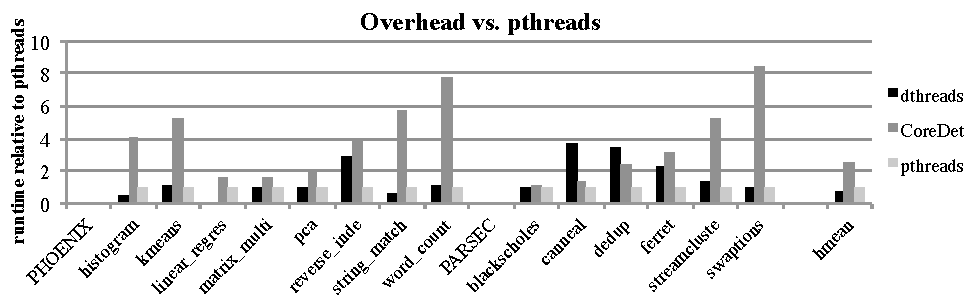
\includegraphics[width=5in]{fig/overhead-figure}
\caption{Normalized execution time with respect to \pthreads{} (lower is better). For 8 of the 14 benchmarks, \dthreads{} runs as fast or faster than \pthreads{}, while providing deterministic behavior.\label{fig:performance}}
}
\end{figure*}

\begin{table*}[!t]
\centering
\begin{tabular}{|l|rrr|l|}
\hline
 & {\bf \small \dthreads{} } & {\bf \small pthreads} & {\bf \small CoreDet} &  \\
{\bf \small Benchmark} & {\bf \small (s)} & {\bf \small (s) } & {\bf \small (s)} & {\bf \small Input} \\
\hline
{\bf \small histogram} & 0.35 & 0.73 & 0.97 & {\bf \small large.bmp} \\
{\bf \small kmeans} & 15.02 & 13.16 & 68.41 & {\bf \small -d 3 -c 1000 -p 100000 -s 1000} \\ 
{\bf \small linear\_regression} & 0.57 & 4.11 & 6.42 &  {\bf \small key\_file\_500MB.txt} \\
{\bf \small matrix\_multiply} & 19.28 & 19.32 & 31.68 & {\bf \small 2000 2000 } \\
{\bf \small pca} & 21.14 & 20.49 & 39.24 & {\bf \small -r 4000 -c 4000 -s 100 } \\
{\bf \small reverse\_index} & 6.53 & 2.06 & 7.85 & {\bf \small datafiles} \\
{\bf \small string\_match} & 1.97 & 3.19 & 18.31 & {\bf \small key\_file\_500MB.txt} \\
{\bf \small word\_count} & 2.37 & 2.17 & 17.17 & {\bf \small word\_100MB.txt} \\
{\bf \small blackscholes} & 9.30 & 9.47 & 10.49 & {\bf \small 8 in\_1M.txt prices.txt} \\
{\bf \small canneal} & 39.82 & 10.41 & 14.74 & {\bf \small 7 15000 2000 400000.nets 128} \\
{\bf \small dedup} & 5.39 & 1.45 & 3.38 & {\bf \small -c -p -f -t 2 -i media.dat output.txt} \\
{\bf \small ferret} & 26.86 & 7.02 & 21.89 & {\bf \small corel lsh queries 10 20 1 output.txt} \\
{\bf \small streamcluster} & 4.61 & 2.74 & 14.33 & {\bf \small 10 20 128 16384 16384 1000 none output.txt 8} \\
{\bf \small swaptions} & 3.88 & 4.18 & 35.21 & {\bf \small -ns 128 -sm 50000 -nt 8} \\
\hline
\end{tabular}
\caption{Benchmarks.\label{tbl:benchmarks}}
\end{table*}

\begin{table*}[!t]
\centering
\begin{tabular}{|l|rrrrr|}
\hline
& {\bf \small Serial Phase} & {\bf \small Transactions} & {\bf \small TransLength} & {\bf \small DirtyPages} & {\bf \small DirtyPages}
\\
{\bf \small Benchmark} & {\bf \small (\% of time)} & {\bf (\#)} & {\bf \small (ms)} & {\bf \small (\#)} & {\bf \small (GB)}\\
\hline
\multicolumn{6}{|c|}{\emph{Phoenix}} \\
\hline
\small \textbf{histogram} & 0 & 23 & 15.47 & 29 & 0 \\
\small \textbf{kmeans} & 0 & 3929 & 3.82 & 9466 & 0.04\\
\small \textbf{linear\_regression} & 0 & 24 & 23.92 & 17 & 0\\
\small \textbf{matrix\_multiply} & 0 & 24 & 841.2 & 3945 & 0.02\\
\small \textbf{pca} & 0 & 48 & 443 & 11471 & 0.04 \\
\small \textbf{reverseindex} & 17\% & 61009 & 1.04 & 451876 & 1.72\\
\small \textbf{string\_match} & 0 & 24 & 82 & 41 & 0 \\
\small \textbf{word\_count} & 1\% & 90 & 26.5 & 5261 & 0.02\\
\hline
\multicolumn{6}{|c|}{\emph{PARSEC}} \\
\hline
\small \textbf{blackscholes} & 0 & 24 & 386.9 & 991 & 0\\
\small \textbf{canneal} & 26.4\% & 1062 & 43 & 3606413 & 13.75\\
\small \textbf{dedup} & 31\% & 45689 & 0.1 & 356589 & 1.36\\
\small \textbf{ferret} & 12.3\% & 484127 & 0.05 & 844184 & 3.21 \\
\small \textbf{streamcluster} & 18.4\% & 130001 & 0.04 & 131992 & 0.50\\
\small \textbf{swaptions} & 0 & 24 & 163 & 867 & 0\\
\hline
\end{tabular}
\caption{Benchmark characteristics.\label{tbl:characteristics}}
\end{table*}


\begin{figure}[!t]
\caption{Scalability.\label{fig:scalability}}
\end{figure}

\subsection{Experimental Environment}
All evaluations are performed on a Intel Core2 Dual-Processor CPU, each
processor is a 4-core 64-bit Xeon running on at 2.33GHZ with 4MB L2 cache. 
The totoal memory for this system is 16GB. The operating system we are using
is CentOs 5.5, with the Linux kernel version 2.6.18-194.17.1.el5. 
Kernel is un-modified to run the experiments.

\subsection{Methodology}

\textbf{Methodology. The machine. The compilers. The benchmarks. How we run
things (drop first, keep next five). Variance - when reported.
Harmonic mean (mention here)? LLVM vs. gcc if necessary. Matching
number of threads to number of cores.}

We evaluate the performance and scalability of \dthreads{} across the
PARSEC~\cite{parsec} and Phoenix~\cite{phoenix-hpca} benchmark suites.
We do not include results for \texttt{bodytrack}, \texttt{fluidanimate}, \texttt{x.264}, 
\texttt{facesim}, \texttt{vips}, \texttt{raytrace} benchmarks from PARSEC, 
since they do not currently work with \dthreads{}.

In order to compare the performance against CoreDet, we are using the
LLVM compiler with ``-O5''
optimizations~\cite{LLVM:CGO04}. Since \dthreads{} does not currently
support 64-bit binaries, all benchmarks are compiled for 32 bit
environments (using the ``-m32'' compiler flag). We run each benchmark
ten times, discard the lowest and highest execution times, and present the
average of the remaining eight.

The performance of CoreDet~\cite{Bergan:2010:CCR:1736020.1736029} is
extremely sensitive to three parameters: granularity in bytes for the
ownership table, quantum size in the number of instructions retired,
and the choice between full serial mode and reduced serial mode. We
compare the performance and scalability of \dthreads{} with the best
possible results that we could obtain for CoreDet---that is, with the
lowest average normalized runtimes---after an extensive search of the
parameter space (six possible granularities and 8 possible quanta, for
each benchmark): the parameters shown here are for a 64-byte
granularity and a quantum size of 100,000 instructions, in full serial
mode.
 
For scalability experiments, we logically disable CPUs using Linux's
CPU hotplug mechanism, which allows us to disable or enable indivdual
CPUs by writing ``0'' (or ``1'') to a special pseudo-file
(\url{/sys/devices/system/cpu/cpuN/online}).

Graph / table / things to do punchlist:

\begin{enumerate}
\item Table of benchmarks (and inputs, if possible), Table~\ref{tbl:benchmarks}.
\item Benchmark characteristics table, Table~\ref{tbl:characteristics}.
\item 8-core numbers for \pthreads{}, \dthreads{}, CoreDet, Figure~\ref{fig:performance}.
\item Scalability graphs for above, Figure~\ref{fig:scalability}.
\item Make sure to report results for \emph{racey}.
\item Relative performance: \dthreads{} and CoreDet, etc. vs. \pthreads{} (T\_pthreads / T\_other)
\item CoreDet vs. \dthreads{} (normalized to \dthreads{}) to show CoreDet overhead.
\item Explanation of what benchmarks we do not run (because of limitations of \dthreads{}): x.264, bodytrack, facesim, fluidanimate.
\end{enumerate}

Benchmark performance. Good except for outliers. Compare to CoreDet.

\subsection{Determinism}
We experimentally verified \dthreads{}' ability to ensure determinism
by executing the \emph{racey} determinism tester~\cite{1508256}, which
is extremely sensitive to memory-level non-determinism. \dthreads{}
reported the same results for 2,000 runs.

\subsection{Performance}
In this section, we compare the performance of \dthreads{} with \texttt{pthreads} and CoreDet.
Those results are showed in Figure~\ref{fig:performance} and Table~\ref{tbl:benchmarks}.
For 8 out of 14 test case, \dthreads{} runs as fast as or faster than \texttt{pthreads} library.
For those benchmarks running faster using \dthreads{}, reasons are listed in the following:
\begin{itemize}
\item Linear\_regression: original program suffers from catastrophic false sharing, \dthreads{} can tolerate the false 
sharing problem, thus provides much better performance. 
\item Histogram, swaptions: they can perform much better by using the multi-process framework only, we are not clear about the reason now. 
\item String\_match: it also suffers from the false sharing problems, which \dthreads{} can avoid that.
\end{itemize}

The following benchmarks run slower using \dthreads{}.  
\begin{itemize}
\item kmeans: kmeans creates over 1000 threads totally. Since default workload is light weight, which is not the case for most applications, 
then the overhead to create one process dominiates the overhead. It is clear that the creation of one process is more expensive than the creation of one thread, but for most applications, thread creation and destruction are rare.
\item Ferret: ferret are using the ``pipeline'' thread model. The first stage relies on external library to 
analyze the image file, which uses substantial unnecessary locks (over 1000). Since \dthreads{} are scheduled based on 
synchronization, which makes most stages serialized.
\item Canneal, Dedup, Reverse\_index: these benchmarks invoke too many pages commit and protection overhead, 
see Table~\ref{tbl:benchmarks} for more details.
\end{itemize}

\subsection{Scalability}

\subsection{Characteristics}

The data showed in Table~\ref{tbl:characteristics} are got from the executions using 8 threads. 
Column 2 shows the percentage of time spending in the serial phase. According to our model (Figure~\ref{phase}), 
all commits and synchronizations are finished in the serial phase. 
The percentage of time spending in serial phase can affect the performance and scalability.

Column 3 examines how many transactions happen in the application and 
column 4 examines the average length of each transaction (ms). 
Remember that all kinds of synchronization, including locks, conditional variable, barrier 
and different thread exit, can close one transaction (\texttt{atomicEnd}).
Since \texttt{atomicEnd} should commit those local changes to 
the shared mapping, in order to create the illusion of share address space, 
which can affect the performance greatly if there are substantial commits in one short transaction. 
For example, \texttt{reverse\_index}, \texttt{dedup}, \texttt{ferret} and \texttt{streamcluster}
have lots of transactions, with transaction length less than 1ms, 
which cause some performance penalty for these applications. 
While those benchmarks with fewer transactions or longer transaction length, they can run almost the same speed or faster than \texttt{pthreads}, like \texttt{histogram} or \texttt{pca}.
In \dthreads{}, longer transaction length can amortize the overhead of memory overhead. 

Column 5 and 6 examines more direct overhead from memory, 
including the memory protection system calls, memory trap and memory commit. 
Here we are using those pages numbers as 
the indication of memory overhead, since \dthreads{}  captures those possible pages modified in one transaction 
by using page protection, 
get the details about changes on one page by comparing the private copy with twinning page and 
commit changes to the shared mapping in the end. 
From the table, we can know that \texttt{canneal} are much slower than that using \texttt{pthreads} since this benchmark 
involves in over 13G memory operations, including creation of private copy and commit to shared copy. According to
our test, copying the 1G memory needs about 0.8 seconds if we are using the memcpy provided by glibc library.

